\chapter{Referencial Teórico}

\lipsum[1-2]

\begin{citacao}
\lipsum[1] \cite[p. ~34]{Huizinga2014}
\end{citacao}

\section{Tema 1}

De acordo com \citeonline{SalenZimmerman2012}, ...

\lipsum[4-7]


\section{Tema 2}

De acordo com \citeonline{SalenZimmerman2012}, ...

\lipsum[4-7]

A figura \ref{fig:kings-landing} representa \emph{King's Landing}, cenário da série \emph{Game of Thromes} reproduzido no Minecraft:

\begin{figure}[h]
	\caption{\emph{The King's Landing} no Minecraft}
	\center
	\label{fig:kings-landing}
	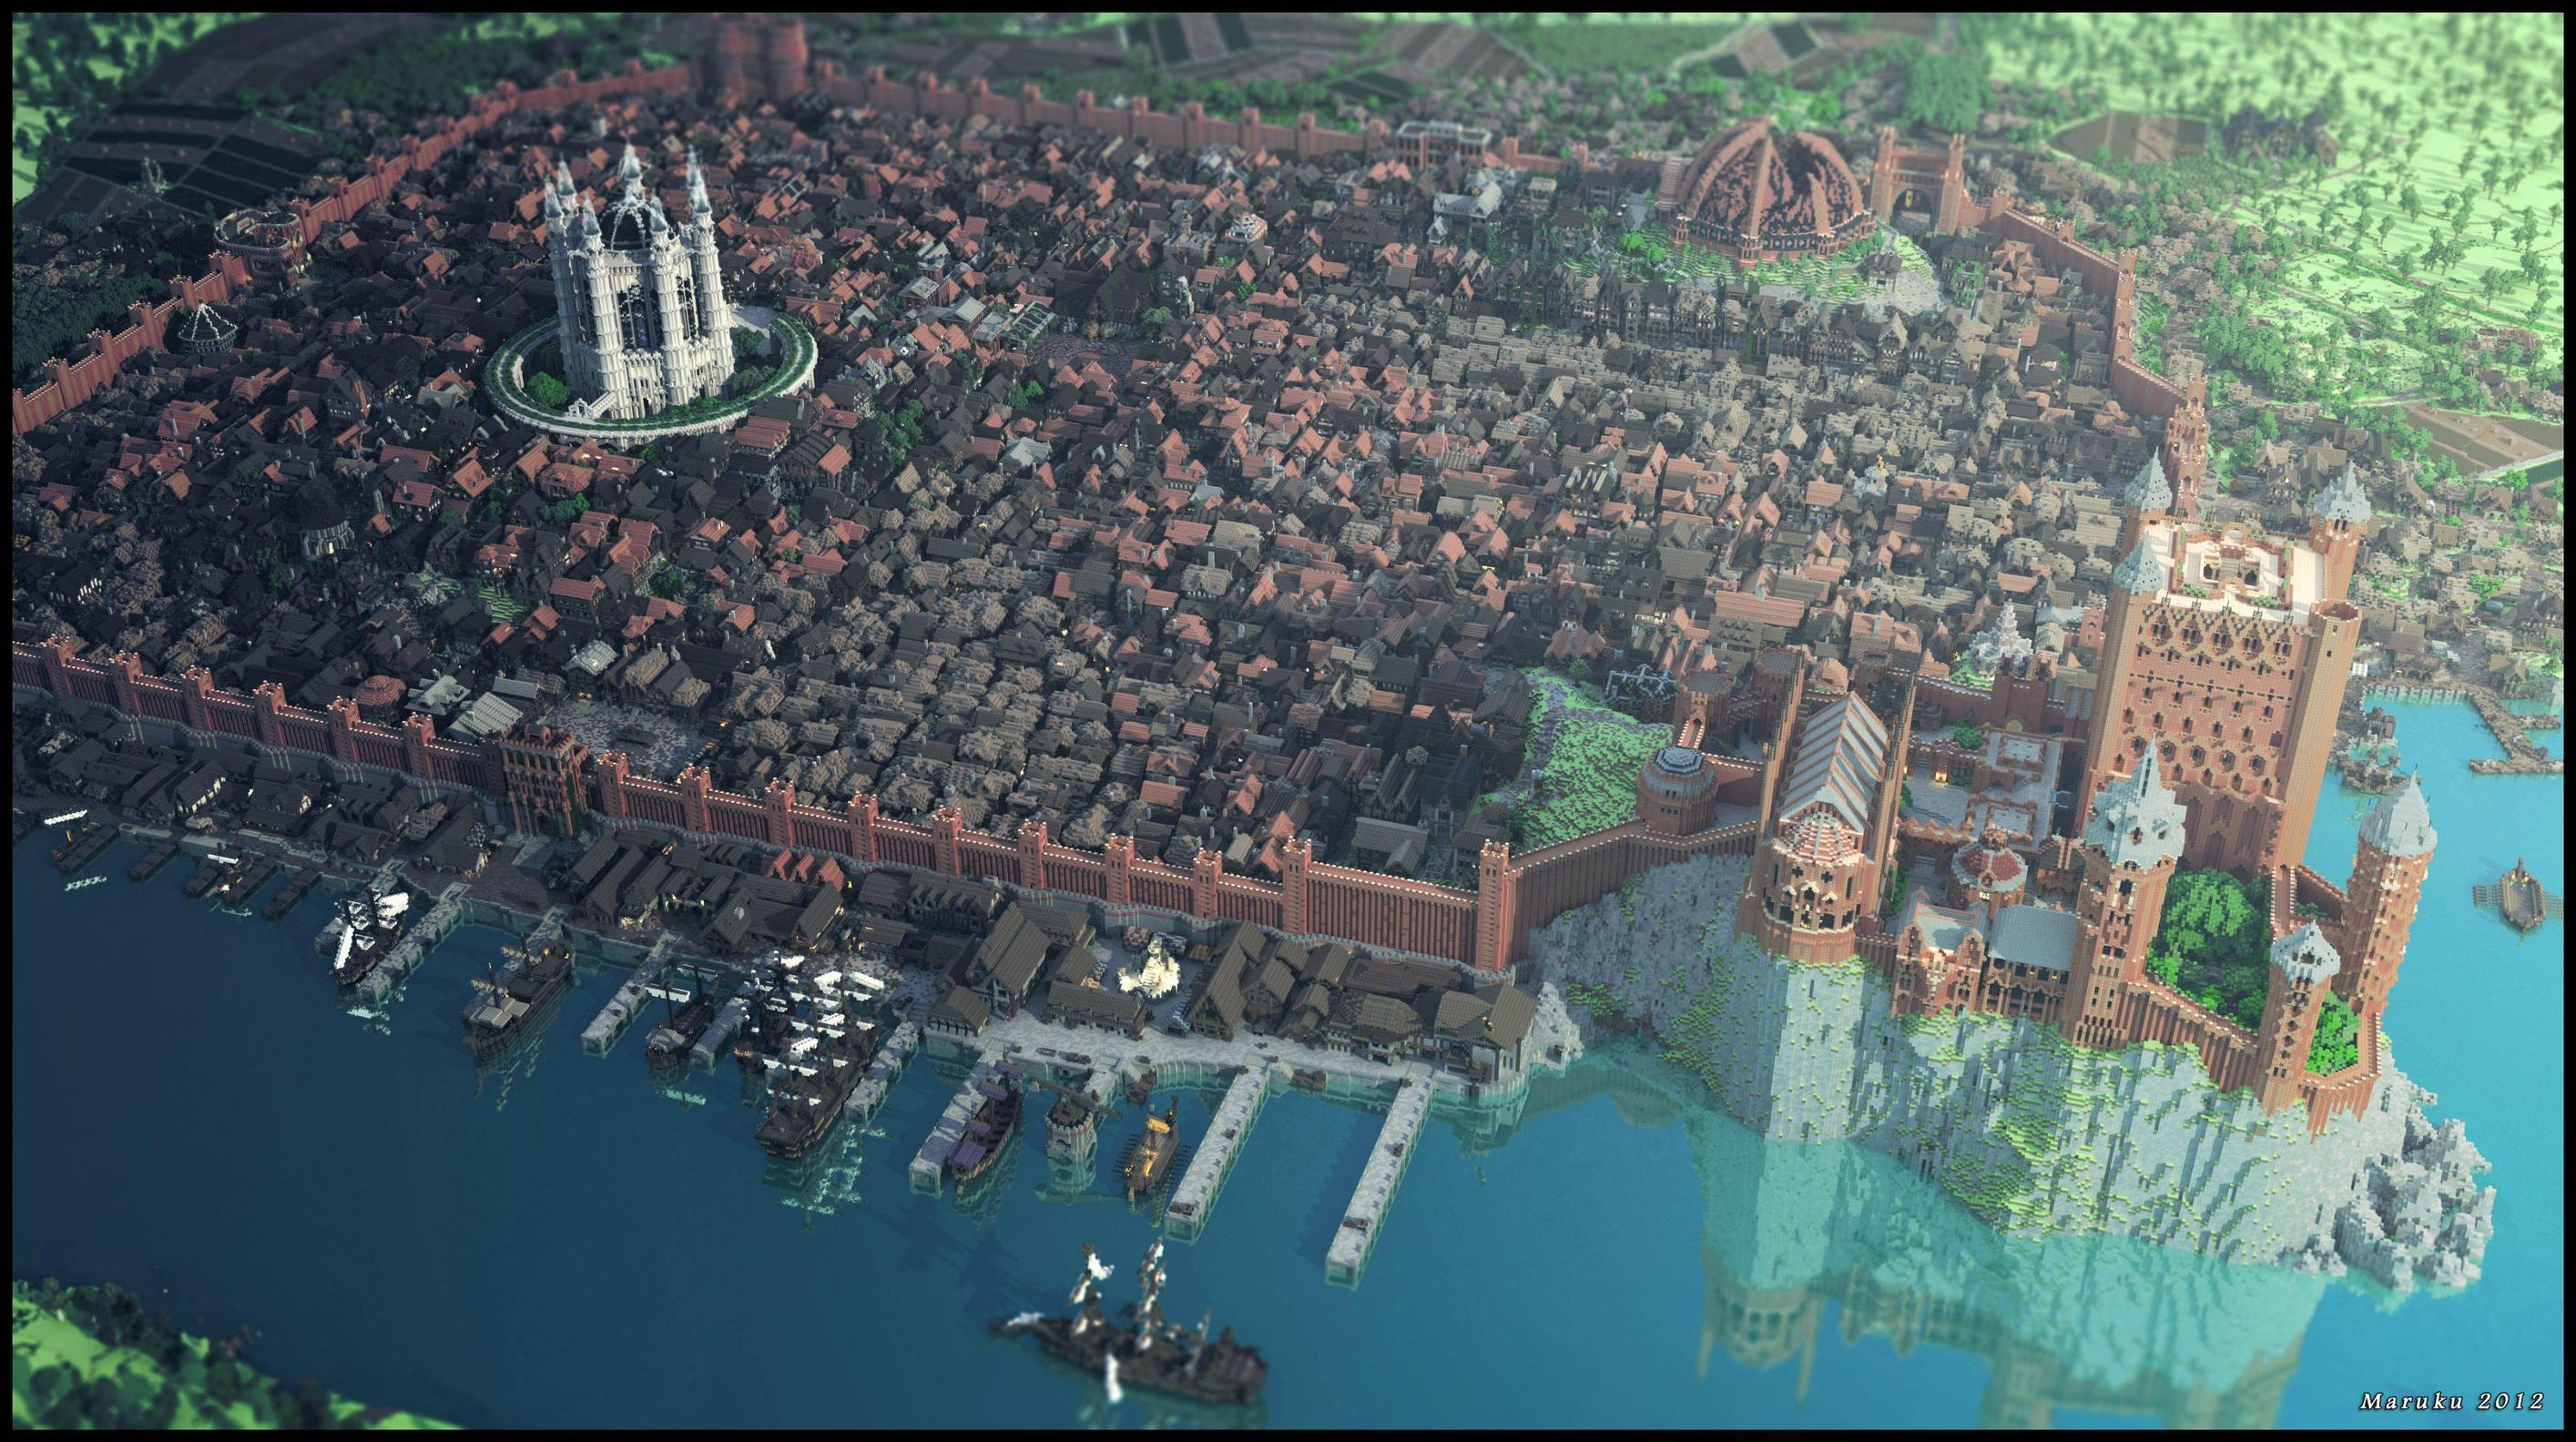
\includegraphics[scale=0.15]{fundamentacao/kings-landing.jpg}
	\fol{Imgur2013}
\end{figure}

\lipsum[10-12]

